\begin{surferPage}[216 Singularitäten]{Flächen mit vielen reellen Singularitäten}
  Wie bereits erwähnt, ist schon für Flächen von Grad $7$ unbekannt, was die
    maximale Anzahl $\mu(7)$ von singulären Punkten darauf ist; man weiß derzeit
    nur, dass $99\le \mu(7) \le 104$ gilt. 

    Daher erstaunt es nicht, dass man für beliebigen Grad $d$ noch weniger
    weiß.
    Sonja Breske, Oliver Labs und Duco van Straten konnten 2005 wenigstens eine
    Konstruktion von S.V.\ Chmutov so verändern, dass das bisher bekannte
    Maximum von Singularitäten, $\mu(d)$, nun auch mit reellen Singularitäten 
    erreicht wird.
    Man weiß daher bisher: 
    \[0,41\bar{6}d^3 \lessapprox \mu(d) \lessapprox 0.44\bar{4} d^3.\]
    Von oben erkennt man schön die Symmetrie der Konstruktion
    und ihren Zusammenhang mit der Frage nach der maximalen Anzahl schwarzer
    Zellen in einem Arrangement von Geraden:
    \begin{center}
      \begin{tabular}{c@{\qquad}c}
        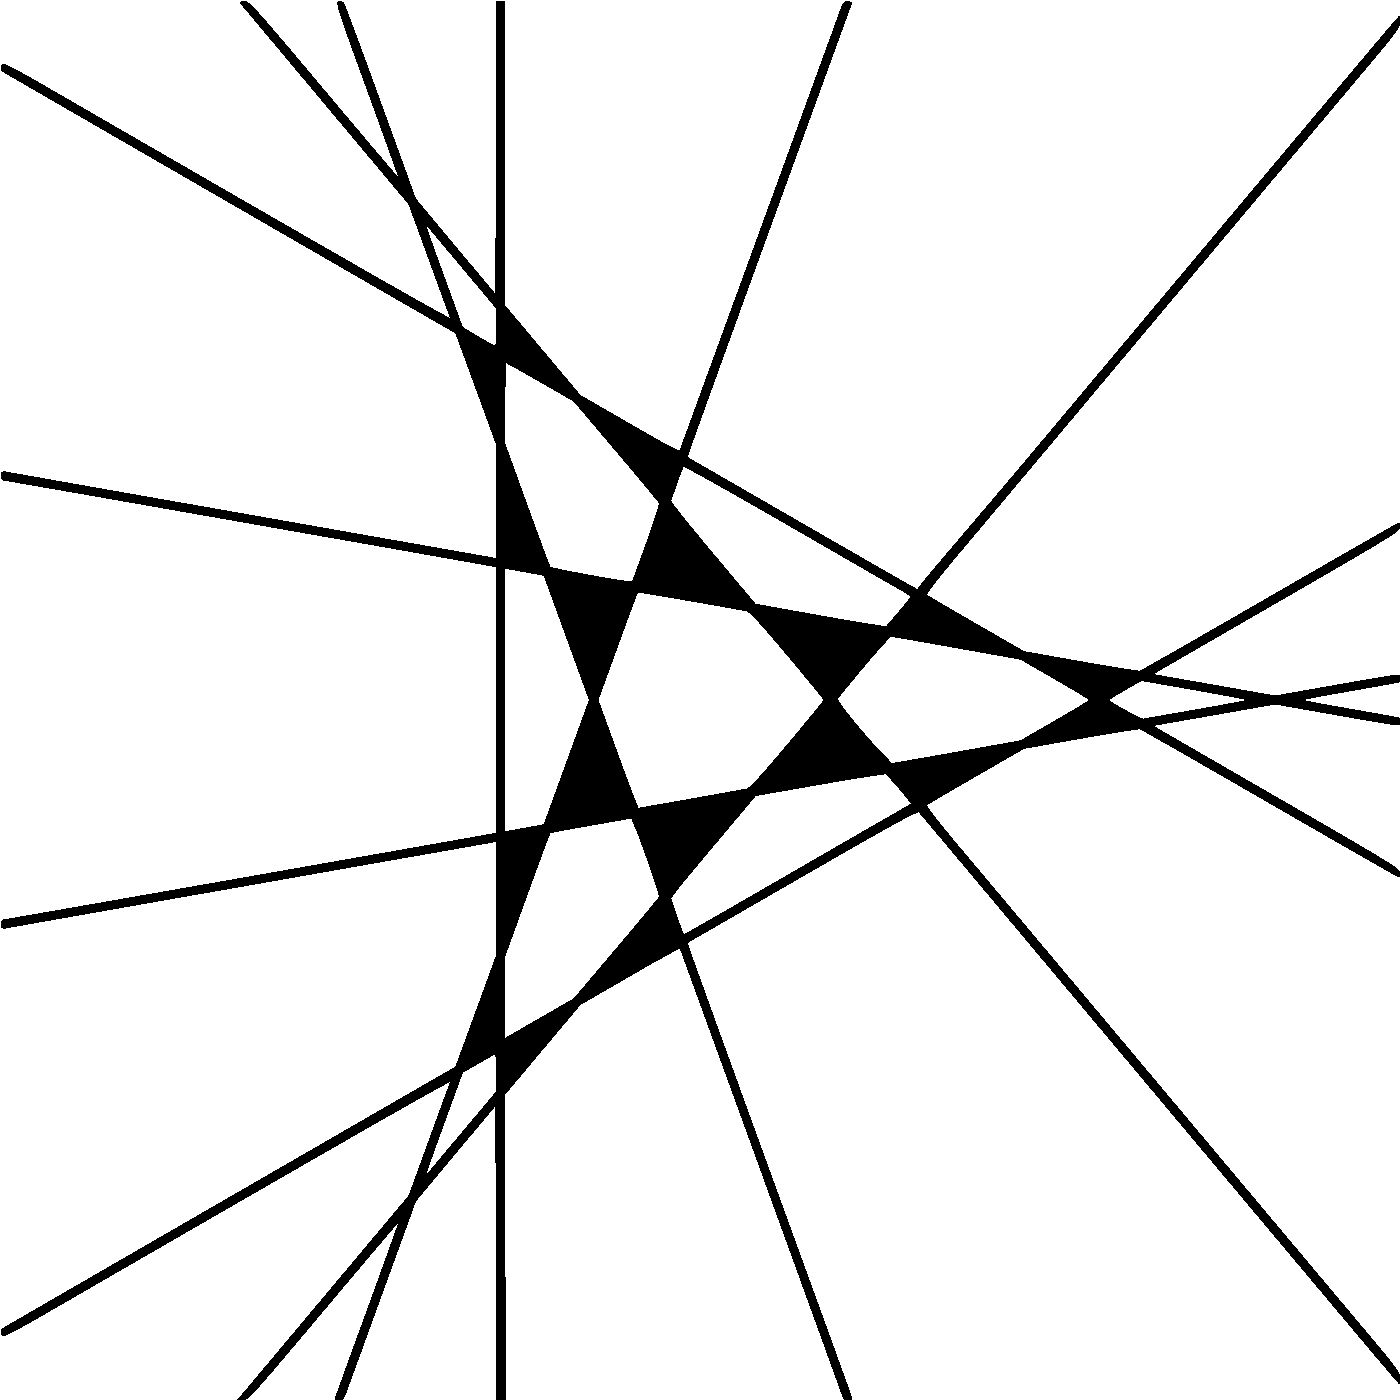
\includegraphics[height=1.5cm]{./../../common/images/vielesing.pdf}
        &
        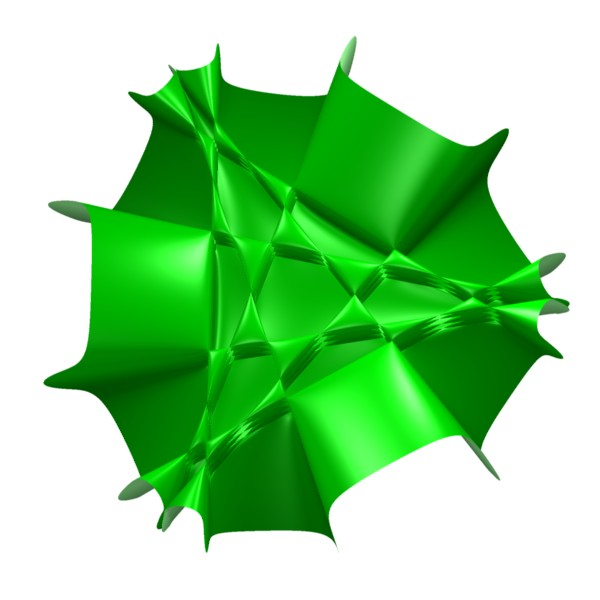
\includegraphics[height=1.5cm]{./../../common/images/p9surface_von_oben}
      \end{tabular}
    \end{center}
\end{surferPage}
